\prechapter{Cambios en modulos del sistema}

\section{Cambios Realizados}
Se ha realizado una serie de cambios en el sistema para mejorar su funcionalidad y flexibilidad. A continuación, se detallan los cambios más importantes:

\subsection{Adición de la Tabla de Normalización}
Se ha añadido una nueva tabla para la normalización de datos. Esta tabla permite mantener la integridad y consistencia de los datos en el sistema.

\subsection{Adición de la Tabla de Filtros}
Se ha añadido una nueva tabla llamada \textbf{Filtros} que permite crear condiciones para la generación de alertas. Esta tabla facilita la configuración de alertas basadas en diferentes criterios y umbrales.

\subsection{Actualización de Diagramas}
Se han actualizado los diagramas de clases y de entidad-relación para reflejar los cambios realizados. A continuación, se muestran los espacios para los nuevos diagramas:

\begin{figure}[h!]
    \centering
    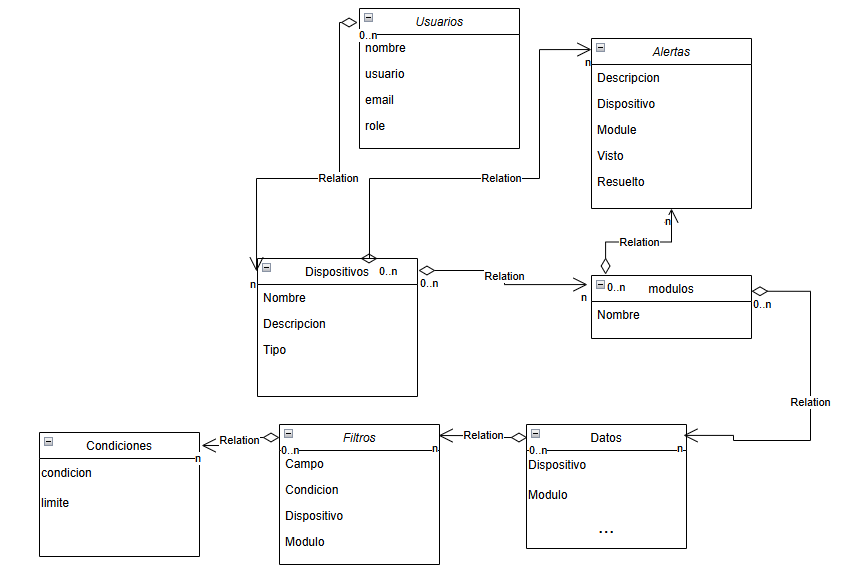
\includegraphics[width=\textwidth]{imagenes/contenido/ClasesActual.png}
    \caption{Nuevo Diagrama de Clases.}
\end{figure}

\begin{figure}[h!]
    \centering
    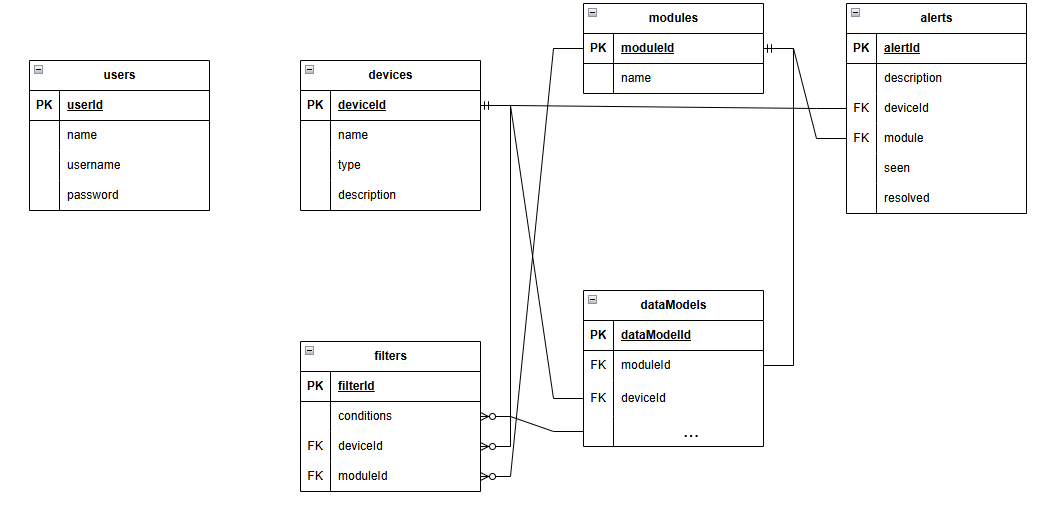
\includegraphics[width=\textwidth]{imagenes/contenido/ERActualizado.png}
    \caption{Nuevo Diagrama de Entidad-Relación.}
\end{figure}

\section{Tablas de Datos}

\subsection{Tabla de Usuarios}
\begin{table}[h!]
    \centering
    \begin{tabular}{|c|c|c|}
    \hline
    \rowcolor[HTML]{FCE8B2} 
    \textbf{Campo} & \textbf{Tipo de Dato} & \textbf{Descripción} \\ \hline
    username & Cadena de texto & Nombre de usuario, único y requerido. \\ \hline
    name & Cadena de texto & Nombre completo del usuario, requerido. \\ \hline
    password & Cadena de texto & Contraseña del usuario, requerida. \\ \hline
    createdAt & Fecha/Hora & Fecha y hora de creación del registro. \\ \hline
    updatedAt & Fecha/Hora & Fecha y hora de la última actualización del registro. \\ \hline
    \end{tabular}
    \caption{Especificaciones de la Tabla de Usuarios.}
\end{table}

\subsection{Tabla de Módulos}
\begin{table}[h!]
    \centering
    \begin{tabular}{|c|c|c|}
    \hline
    \rowcolor[HTML]{FCE8B2} 
    \textbf{Campo} & \textbf{Tipo de Dato} & \textbf{Descripción} \\ \hline
    name & Cadena de texto & Nombre del módulo, requerido. \\ \hline
    \end{tabular}
    \caption{Especificaciones de la Tabla de Módulos.}
\end{table}

\subsection{Tabla de Filtros}
\begin{table}[h!]
    \centering
    \begin{tabular}{|c|c|c|}
    \hline
    \rowcolor[HTML]{FCE8B2} 
    \textbf{Campo} & \textbf{Tipo de Dato} & \textbf{Descripción} \\ \hline
    field & Cadena de texto & Campo sobre el que se aplica el filtro, requerido. \\ \hline
    conditions & Arreglo & Conjunto de condiciones para el filtro. \\ \hline
    device & ObjectId & Referencia al dispositivo, requerido. \\ \hline
    module & ObjectId & Referencia al módulo, requerido. \\ \hline
    createdAt & Fecha/Hora & Fecha y hora de creación del registro. \\ \hline
    updatedAt & Fecha/Hora & Fecha y hora de la última actualización del registro. \\ \hline
    \end{tabular}
    \caption{Especificaciones de la Tabla de Filtros.}
\end{table}

\subsection{Tabla de Dispositivos}
\begin{table}[h!]
    \centering
    \begin{tabular}{|c|c|c|}
    \hline
    \rowcolor[HTML]{FCE8B2} 
    \textbf{Campo} & \textbf{Tipo de Dato} & \textbf{Descripción} \\ \hline
    name & Cadena de texto & Nombre del dispositivo, requerido. \\ \hline
    type & Cadena de texto & Tipo de dispositivo, requerido. \\ \hline
    description & Cadena de texto & Descripción del dispositivo, requerida. \\ \hline
    createdAt & Fecha/Hora & Fecha y hora de creación del registro. \\ \hline
    updatedAt & Fecha/Hora & Fecha y hora de la última actualización del registro. \\ \hline
    \end{tabular}
    \caption{Especificaciones de la Tabla de Dispositivos.}
\end{table}

\subsection{Tabla de Alertas}
\begin{table}[h!]
    \centering
    \begin{tabular}{|c|c|c|}
    \hline
    \rowcolor[HTML]{FCE8B2} 
    \textbf{Campo} & \textbf{Tipo de Dato} & \textbf{Descripción} \\ \hline
    description & Cadena de texto & Descripción de la alerta, requerida. \\ \hline
    device & ObjectId & Referencia al dispositivo, requerido. \\ \hline
    module & ObjectId & Referencia al módulo, requerido. \\ \hline
    seen & Booleano & Estado de la alerta (vista o no vista). \\ \hline
    resolved & Booleano & Estado de resolución de la alerta. \\ \hline
    createdAt & Fecha/Hora & Fecha y hora de creación del registro. \\ \hline
    updatedAt & Fecha/Hora & Fecha y hora de la última actualización del registro. \\ \hline
    \end{tabular}
    \caption{Especificaciones de la Tabla de Alertas.}
\end{table}

\subsection{Tabla de Invernaderos}
\begin{table}[h!]
    \centering
    \begin{tabular}{|c|c|c|}
    \hline
    \rowcolor[HTML]{FCE8B2} 
    \textbf{Campo} & \textbf{Tipo de Dato} & \textbf{Descripción} \\ \hline
    module & ObjectId & Referencia al módulo, requerido. \\ \hline
    device & ObjectId & Referencia al dispositivo, requerido. \\ \hline
    Sensores & Objeto & Conjunto de sensores con sus propiedades. \\ \hline
    createdAt & Fecha/Hora & Fecha y hora de creación del registro. \\ \hline
    updatedAt & Fecha/Hora & Fecha y hora de la última actualización del registro. \\ \hline
    \end{tabular}
    \caption{Especificaciones de la Tabla de Invernaderos.}
\end{table}